% Sudut 135 derajat dengan busur — pakgun.gezytech.web.id
% Kompilasi: pdflatex tikz-sudut-busur-derajat.tex
\documentclass[tikz,border=8pt]{standalone}
\usepackage{amsmath}
\usetikzlibrary{angles, quotes}
\definecolor{bgdark}{HTML}{171D2B}
\definecolor{aksen}{HTML}{F7B538}
\begin{document}
\pagecolor{bgdark}
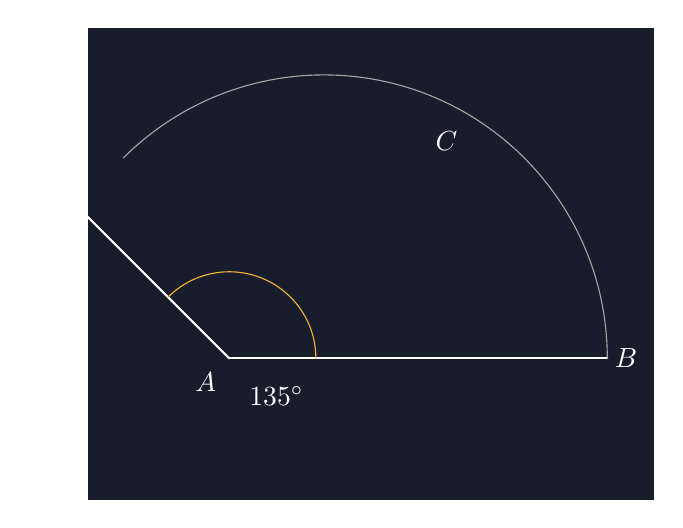
\begin{tikzpicture}[scale=1.2, line cap=round]
  \fill[bgdark] (-1.5,-1.5) rectangle (4.5,3.5);
  \coordinate (A) at (0,0);
  \coordinate (B) at (4,0);
  \coordinate (C) at (135:3);
  \draw[thick, white] (A) -- (B);
  \draw[thick, white] (A) -- (C);
  \draw[gray!70] (B) arc[start angle=0, end angle=135, radius=3];
  \pic[draw, aksen, angle eccentricity=1.4, angle radius=1.1cm]
    {angle = B--A--C};
  \node[white] at (0.5,-0.4) {$135^\circ$};
  \node[white, fill=bgdark, inner sep=1pt] at (2.3,2.3) {$C$};
  \node[white, fill=bgdark, inner sep=1pt] at (4.2,0) {$B$};
  \node[white, fill=bgdark, inner sep=1pt] at (-0.25,-0.25) {$A$};
\end{tikzpicture}
\end{document}
